\documentclass[letterpaper,english]{scrartcl}
\usepackage[T1]{fontenc}
\usepackage{graphicx}
\usepackage{float}
\graphicspath{ {img/} }

\begin{document}
\title{Undergraduate Independent Research Report}
\subtitle{Predicting Bus Occupancy}
\author{Daniel Bordak, Erin Corrado, Revan Sopher, and Ashley Weaver}

\maketitle

\section*{Abstract}
\begin{abstract}
In this study we address the problem of programatically predicting bus occupancy.
We approach this in two ways: by using publically available GPS positions to calculate stop time, and by using promiscuous Wi-Fi to count devices.
While the stop time approach proved unfruitful due to a lack of correlation between stop time and occupancy, ...
\end{abstract}

\section*{Motivation}

Due to the periodic nature of class schedules, students at Rutgers tend to move between campuses at similar times during the day.
This leads to predictable migratory patterns. However, the bus schedule does a poor job of taking this into account: on Livingston campus, for example, the College Ave/Livingston buses circulate consecutively yet are nearly empty, while the Busch/Livingston buses are less frequent and often packed to capacity.
The aim of this project is to develop a system for better predicting demand for buses, such that an empirical argument for the optimization of the bus schedule might be made.

\section*{Approach}

In order to facilitate simultaneous contributions from all four team members, we approached the problem in two manners: by collecting data ourselves, and by using transit times.
Two students worked on each approach, planning to combine results into a single prediction method.

	\subsection*{Stop Length Inference}

	In this approach, we planned to use the logical correlation between the amount of time a bus spends at a stop and the amount of people riding: the idea is that as a bus nears capacity, stops will be longer due to the larger volume of riders entering and exiting.
	Every Rutgers bus periodically updates an internet source with its position, velocity, and destination.
	We first tried to measure the strength of this correlation; if we could prove a strong positive correlation, then we would use the publicly available bus travel data to measure length of stops, and therefore occupancy.
	Although this method inherently depends on a weaker correlation than the number of smartphones, by running the analysis on a log of travel data we could predict occupancy across a significantly larger domain and for no cost.

	\subsection*{Promiscuous WiFi}

	In this approach, we use the inherent correlation between amount of smart phones on the bus and amount of people on the bus.
	We used a laptop running Linux, equipped with a standard wireless card and a GPS sensor.
	The computer runs the wireless card in monitor mode, allowing it to process all packets it receives regardless of destination. It logs the headers of these packets to file, with current time.
	The computer also logs GPS coordinates.

\section*{Results}

\subsection*{Stop Length Inference}
	In order to establish a correlation between stop length and bus occupancy, we followed a bus on its circuit, recording data on its stops.
	\begin{figure}[H]
	\includegraphics[width=11cm]{stop3}
	\centering
	\end{figure}
	As we quickly found, stop length does not appear to have any correlation to occupancy.
	This makes sense, because the amount of sedentary riders does not cause slowdowns, rather the interesting metric is the amount of people entering or exiting the bus.

	\begin{figure}[H]
	\includegraphics[width=11cm]{stop1}
	\centering
	\end{figure}

	Plotting the net occupancy change over stop length was also inconclusive, as the longer stops could be either positive or negative changes.
	From stop timings alone, we would not be able to predict the direction of change.

	\begin{figure}[H]
	\includegraphics[width=11cm]{stop2}
	\centering
	\end{figure}

	Net change, however, shows a stronger correlation, confirming our hypothesis that high rider throughput causes delays.
	Net change is not a useful metric on its own, but if it could be proven that certain bus stops entertained mostly one of boardings or descents, we could predict the sign of the change and thus the occupancy changes over time.

	%TODO:
	\begin{figure}[H]
	GRAPH OF CHANGE AT SINGLE STOP GOES HERE
	\centering
	\end{figure}

	A cursory analysis of this idea suggested that bust stops are not in fact characterized by one of either boardings or descents.
	Thus, we abandoned this line of inquiry.


\subsection*{Promiscuous WiFi}
	To collect data, we put the wireless card into Monitor mode and ran the following:
	\begin{verbatim}
		tcpdump -e
	\end{verbatim}
	This logs the MAC addresses of every packet that the wireless card sees, thus uniquely identifying every active device in the area.
	We followed a bus on its route, logging packets and stop times.

	\begin{figure}[H]
	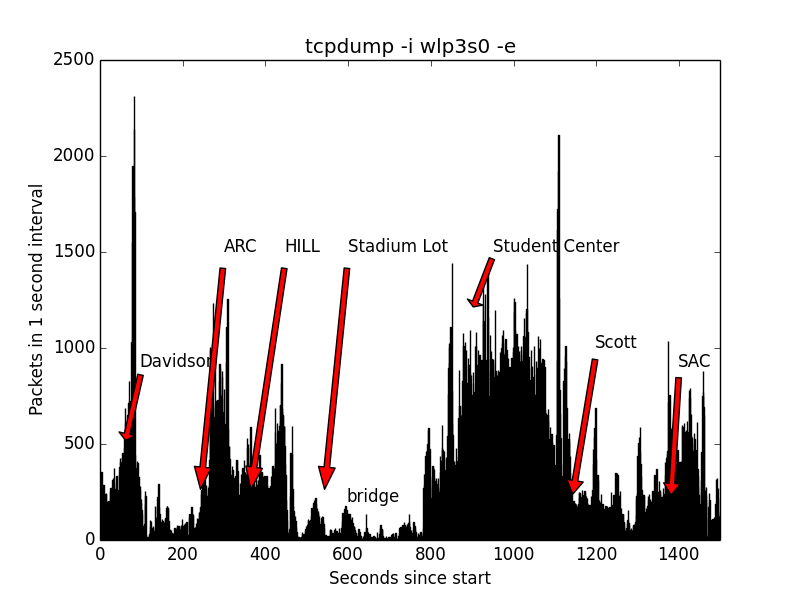
\includegraphics[width=11cm]{packets}
	\\TODO: swap out plot for new data
	\centering
	\end{figure}

	Plotting the number of packets in a histogram with one second bins, we see that there is visible differences between stops.
	There are a few extreme spikes in network traffic, which can be ignored.
	However, this data alone does not establish correlation between traffic and occupancy; since the range of the wireless card extends beyond the bus, there will be considerable noise.
	\\
	tcpdump also records the strength of signals, so we can choose to ignore packets below a certain decibel strength:

	\begin{figure}[H]
	\includegraphics[width=11cm]{strength}
	\\TODO: swap out plot for new data
	\centering
	\end{figure}

	Additionally, we switched out "number of packets" for "number of unique MAC addresses".

	\begin{figure}[H]
	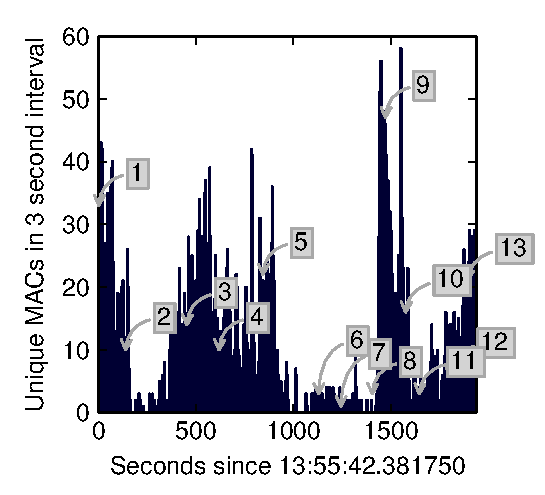
\includegraphics[width=11cm]{unique}
	\\TODO: swap out plot for new data, remake with strength cutoff
	\centering
	\end{figure}

	In order to establish which devices were on the bus, we can also plot the time of the first and last occurance of each device:

	\begin{figure}[H]
	%\includegraphics[width=11cm]{}
	\\TODO: make plot
	\centering
	\end{figure}

	TODO: ANALYSIS


\section*{Future Work}
The largest problem with the interception of packets is outside noise.
To address this, we would like to install an access point on the bus, with the same SSID as the campus Wi-Fi such that smart phones would automatically connect.
We could then listen only to communications with this access point, eliminating outside traffic.
\\
Optimally, the routers would be officially installed, and serve mobile data. This is naturally expensive and thus unlikely. Any unofficial access points installed would be an explicit violation of the terms of use of the Rutgers networks, and thus unfeasible as well.
\\
\\
We could also replace the laptop in our setup with a smaller unit to be installed in the busses, to collect for longer periods of time. Running several of these units would allow us to collect enough data to make occupancy predictions.

\end{document}
